%%%%%%%%%%%%%%%%%%%%%%%%%%%%%%%%%%%%%%%%%%%%%%%%%%%%%%%%%%%%%%%%%%%%%%%%
%                                                                      %
%     File: Thesis_Results.tex                                         %
%     Tex Master: Thesis.tex                                           %
%                                                                      %
%     Author: Andre C. Marta                                           %
%     Last modified :  2 Jul 2015                                      %
%                                                                      %
%%%%%%%%%%%%%%%%%%%%%%%%%%%%%%%%%%%%%%%%%%%%%%%%%%%%%%%%%%%%%%%%%%%%%%%%

\chapter{Application to Deep Learning}
\label{chapter:application}

\section{Deep Learning Overview}
\label{sec:DLO}
Deep Learning (DL) is a subset of the large family of Machine Learning methods. Also known as deep structured learning or hierarchical learning, this type of algorithm is based on artificial neural networks and can be utilized for supervised, semi-supervised, and unsupervised learning \cite{bengio_representation_2013} \cite{schmidhuber_deep_2015}.

Biological systems inspired the creation of Artificial Neural Networks (ANN), in which Deep Learning architectures are built on top. This information-processing and distributed communications type of network work by mimicking a simplistic biological brain where the interconnection between the neurons is static and symbolic \cite{marblestone_toward_2016}. 

Different deep learning architectures are being developed, such as convolutional neural networks (CNN), recurrent and Recursive neural networks (RNN), and unsupervised pre-trained networks (UPT). These have been applied to a diversity of fields, including computer vision, speech and audio recognition, natural language processing, bioinformatics, and others. In such applications, deep learning algorithms are being able to achieve comparable and, in some cases, superior results to humans experts \cite{noauthor_googles_nodate}.

\begin{figure}[!htb]
  \centering
  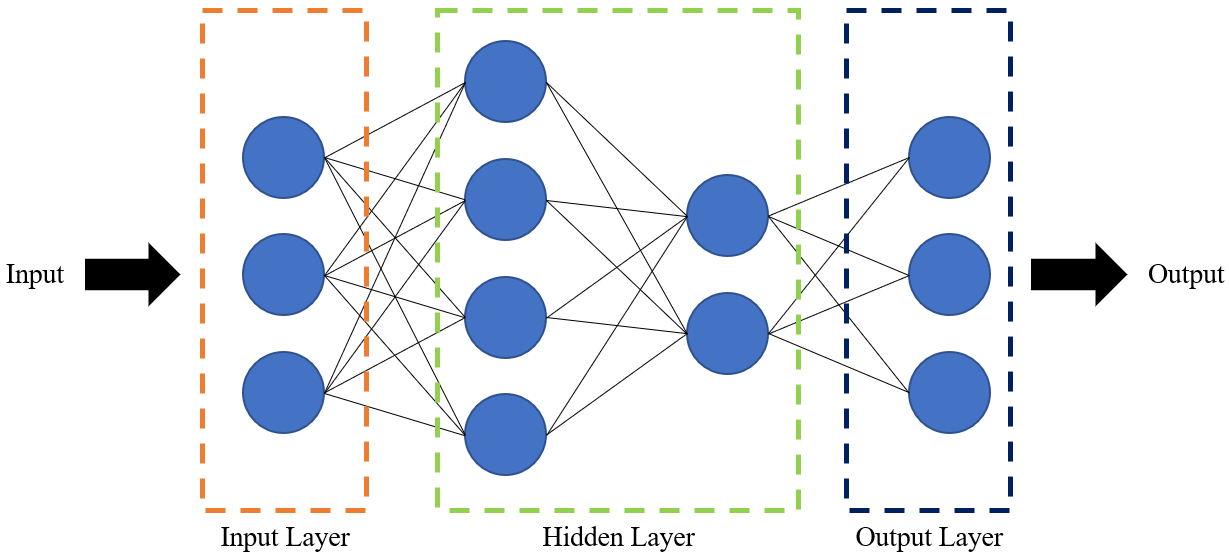
\includegraphics[width=0.75\textwidth]{Figures/DL/DNNarch.png}
  \caption[]{ Modelofafully-connectedfeedforwardnetwork.}
  \label{fig:DNNarch}
\end{figure}


\subsection{Deep Neural Network}
The unitary element of a deep neural network (DNN) is the artificial neuron. This element can be mathematically modeled by a set of multiplications and summations, as shown in Equation \ref{eq:neuron}, where $W_i$ represents the weight and $b$ the bias applied on artificial each neuron.

\begin{equation}
\label{eq:neuron}
    Y = \sum_{i=1}^{n} W_iX_i+b
\end{equation}

One of the significant benefits of deep neural networks is their ability to capture not linear relationships between the input parameters. For that, an activation function is attached to each neuron, helping him to handle scenarios where problems are not linearly separated \cite{dong_dnnmark:_2017}. The most common non-linear activation functions are  hyperbolic tangent (tanh) \cite{orr_neural_1998}, Rectified Linear Unit (ReLU) \cite{orr_neural_1998} and sigmoid \cite{orr_neural_1998}. The architecture of the deep neural network is the combination of the linear transformations performed by the neurons plus the non-linear activation functions.

A neural network is composed of arrangements of neurons and activation functions in layers. Each layer is responsible for applying a series of transformations to the data accordingly to the weight and bias value stored in each artificial neuron. A deep neural network is composed of at least three layers, the input layer, with a number of neurons equal to the input size, at least one hidden layer, being this the distinguishing characteristics of a DNN, and an output layer with the number of neurons equal to the output size. The different organization of the layers in number size, type of operation and number of connections of layers defines the type and architecture of the DNN.

\subsection{Training and Inference}
The mathematical description of the  DNN training process is equivalent to treat the network as a loss function $L$, Equation \ref{eq:loss}, where inputs $X$, outputs $Y$ and the network's parameters weights - $W$ and bias $b$ are function arguments. The objective of the training session is to optimize the in-network parameters of $W$ and $b$ to minimize the overall loss.

\begin{equation}
    \label{eq:loss}
    (W,b) = \arg\min_{W} L(X,Y,W,b)
\end{equation}

The DNN training is an iterative process, where at the end of each iteration, a loss value is computed, and the set of in-network parameters is updated. This loss value represents how well are the input parameters being modeled by the network. It is expected that with the number of training iterations, the loss value reduces and converges to a minimum, at which the model accuracy prediction will be at its maximum. At this point, the training session can be stopped.

The most common method for the parameters update is the Stochastic Gradient Descent (SGD) algorithm, Equation \ref{eq:update}, an iterative algorithm that, after processing mini-batches of the training data, computes new weights and bias for each neuron. 

\begin{equation}
    \label{eq:update}
    W_{i+1} \xleftarrow{} W_i - \alpha \sum_{n=1}^{m}\frac{\partial L}{\partial W_i}
\end{equation}

In Equation \ref{eq:update}, $m$ represents the number of mini-batches, $W_i$ the current parameter, $W_{i+1}$ the update parameter, $\alpha$ the learning rate and $\frac{\partial L}{\partial W_i}$ the partial derivative of the loss function $L$ in order to the parameters. This last of the equation is obtained by applying the derivative chain rule in a backward-cascade fashion with respect to inputs, outputs, and parameters of each DNN layer.

Each iteration of the training process is composed of forward and backward propagation. On the forward propagation, the loss function for the current in-network parameters is evaluated, computing the loss value. By performing the backward propagation, the partial derivative $\frac{\partial L}{\partial W_i}$ of each of the parameters is obtained to apply the SGD algorithm. 

The inference or prediction process corresponds to performing a forward propagation, with the intended inputs, on a previously trained neural network. At the output layer, a set of values or probabilities are computed, corresponding to the prediction that the model gave to the given inputs.

\section{Benchmarks}

For the creation of the novel DVFS aware mechanism, three types of benchmarking applications are going to be needed. In the first stage, the characterization of non-conventional DVFS parameters starts by analyzing simple kernels where different parts of the GPU architecture are stressed, and the effects of combine work types are tested. On the second stage, The simple GPU kernels are combined, forming abstract and independent kernels that represent the variety of work that is performed on the many layer types that compose a DNN model. The last benchmarks, where the complete DVFS aware mechanism is tested, are the fully-fledged state of the art deep neural networks models used nowadays in the use cases stated at Section \ref{sec:DLO}.

\subsection{Fundamental Analysis}
%State different examples of kernels (utilizar os que o João Guerreiro utilizou nos papers de modeling and decompling e GPGPU Power Modeling)

The fundamental analysis and characterization of the GPU are done by running and profiling simple benchmarks that stress the different components of the GPU architecture. Following the strategy used by Guerreiro \textit{et al.} in \cite{guerreiro_gpgpu_2018} \cite{guerreiro_modeling_2019}, a set of benchmarks are devised that fit inside of six categories: arithmetic, special units, branch, shared memory, L2 cache and DRAM.  Listings 3.1 to 3.6 exemplify the skeleton of each category of benchmarks.

Listing 3.1 exercises the arithmetic part of the CU, by performing sequences of multiplications and sums, with data presented on each CU registers. By changing the DATA\_TYPE parameter between int,  float and double, the effects of the type of operand and increased precision can be studied. The benchmark execution starts by each thread, loading a value from the global memory to its registers. It is followed by a variable sequence of size \textit{N} of arithmetic operations followed by placing the computed value, back on the global memory. The variation of \textit{N} allows for the studied of the data utilization rate (number of instructions performed to each pair of load/store instructions).


Listing 3.2 exercises special arithmetic units devised to compute non-linear functions (as the ones used by deep learning applications). Similarly to Listing 3.1, this benchmark starts by loading a value from the global memory, then performs a sequence of size \textit{N} of arithmetic operations and it ends by storing the value back on the global memory.

\noindent\begin{minipage}{.45\textwidth}
\begin{lstlisting}[language=C, caption={Int, SP, DP Code}]
DATA_TYPE r0, r1, r2, r3;

r0=A[threadId]; 
r1=r2=r3=r0; 
for (int i=0;i<N;i++) { 
    r0 = r0 * r0 + r1;  
    r1 = r1 * r1 + r2; 
    r2 = r2 * r2 + r3;  
    r3 = r3 * r3 + r0; 
} 
B[threadId]=r0;
\end{lstlisting}
\end{minipage}\hfill
\begin{minipage}{.45\textwidth}
\begin{lstlisting}[language=C, caption={SF Code}]
DATA_TYPE r0, r1, r2, r3;

r0=A[threadId]; 
r1=r2=r3=r0; 
for(int i=0;i<N;i++) {  
    r0 = log(r1);  
    r1 = cos(r2);  
    r2 = log(r3);  
    r3 = sin(r0);
} 
B[threadId]=r0;
\end{lstlisting}
\end{minipage}

Listing 3.3 studies the influence of branches on the code, that will affect the scheduling of the threads running on each CU. Listing 3.4 explicitly stresses the memory subsystem by using shared memory to allow communication between threads running on the same CU. Here, each thread consecutively performs a load and a store to the shared memory. The addresses used by each thread were chosen to minimize bank conflicts on both operations.


\noindent\begin{minipage}{.4\textwidth}
\begin{lstlisting}[language=C, caption={Branches Code}]
DATA_TYPE r0, r1, r2, r3;

r0=A[threadId]; 
r1=r2=r3=r0; 
for(int i=0;i<N;i++) {  
    r0 = r0 * r0 + r1;  
    if( r0 > 0)
        r1 = r1 * r1 + r2; 
    else 
        r1 = r3 * r3 - r2; 
    r0 = r3 * r3 + r0; 
} 
B[threadId]=r0;
\end{lstlisting}
\end{minipage}\hfill
\begin{minipage}{.55\textwidth}
\begin{lstlisting}[language=C, caption={Shared Memory Code}]
__shared__ DATA_TYPE shared[THREADS]; 
DATA_TYPE r0; 

for(int i=0;i<COMP_ITERATIONS;i++) {  
    r0 = shared[threadId];      
    shared[THREADS - threadId - 1] = r0;
}
\end{lstlisting}
\end{minipage}

To test the L2 cache, the benchmark in Listing 3.5 performs memory transfers between large arrays (sufficiently large to not fit on the lower cache level). Listing 3.6 stresses the DRAM with a benchmark with a similar structure to Listing 3.1. This benchmark uses a lower number of arithmetic instructions per loop iteration and a smaller value of \textit{N} in order for the threads to spend less time inside of CUs, resulting in higher utilization of the DRAM.

\noindent\begin{minipage}{.55\textwidth}
\begin{lstlisting}[language=C, caption={L2 Cache Code}]
DATA_TYPE r0;

for(int i=0;i<COMP_ITERATIONS;i++) {      
    r0 = cdin[threadId];      
    cdout[threadId]=r0;
} 

cdout[threadId]=r0;
\end{lstlisting}
\end{minipage}\hfill
\begin{minipage}{.4\textwidth}
\begin{lstlisting}[language=C, caption={DRAM Code}]
DATA_TYPE r0, r1;

r0=A[threadId]; 
r1=r0; 
for (int i=0;i<N;i++) {  
    r0 = r0 * r0 + r1;  
    r1 = r1 * r1 + r0; 
} 
B[threadId]=r0
\end{lstlisting}
\end{minipage}


A second level of benchmarks is devised by performing linear combinations of the different benchmarks proposed. This will allow for the characterization of the cross-influence of the different GPU components together.





\subsection{DNN Primitives Analysis}
%Use the DNNMark \cite{dong_dnnmark:_2017} benchmark to tested the gained insights from the simple kernels to automatically optimize the DNN layers first independently, then in more complex arrangements.

Targeting the objective of improving the runtime of complete deep learning models, the second set of benchmarks are composed of DNN primitives. These primitives consist of an intermediary layer of characterization since they consist of kernels that perform the same operations as the benchmarks proposed in 3.2.1, however with the objective of performing the operations involved in deep learning. 

In this section, the DNNMark benchmark introduced by Dong \textit{et al.} \cite{dong_dnnmark:_2017} is used. DNNMark suite consists of a collection of deep neural networks primitives with configurable parameters, such as convolution, pooling, local response normalization, activation fully connected and softmax. Each primitive can be used independently or together. This allows for the characterization of each DNN layer and the interlayer influence.



\subsection{Complete Architectures}
\subsubsection{CNN}
\subsubsection{RNN}
\subsubsection{UPT}
GAN - generative adversarial networks

Auto-Encoders - variational autoencoders

\section{Feasibility Assessment}
To assess the viability of the claim made in Chapter 1, that there are more viable and efficient sets of voltage and frequency that can be employed when Imprecision Tolerant applications are being run, a set of experiments were devised to test the order of magnitude of the energy savings and what are the impacts of working in not default voltage and frequency settings. Accordingly, this chapter starts by presenting the experimental setup in Section \ref{section:experimental_setup}, namely the benchmark application and how was it developed and the GPU devices where the tests were executed. Afterwords, Section \ref{section:dvfseffects} presents some interesting results related to the execution of the application with not default GPU parameters.


\subsection{Experimental setup}
\label{section:experimental_setup}

To experimentally show the possible gains achieved when working in the setup presented before, an Artificial Neural Network is executed on a GPU, and in each run, the pair of frequency and voltage is adjusted. This section presents the application chosen to perform the preliminary tests, followed by a description of the GPU device where the experiments were conducted.

To evaluate the energy gains on an imprecision tolerant application, a convolutional neural network (CNN) was used. Convolutional neural networks are a class of artificial neural networks that are most commonly used to analyze images and video to perform image classification. The training of the model, minimization of the loss function, is a convergence process, making this type of applications imprecision tolerent, since small errors on the model training can still lead to the finding of an locally optimal solution.
The developed CNN classifies the MNIST dataset [link to mnist], a set of 60000 train and 10000 test handwritten digits. The CNN was developed using PyTorch [link to pytorch]. Pytorch is an open source machine learning library primarily developed by Facebook's artificial intelligence research group. It is a free and open-source  software released under the Modified BSD licence [link to this claim]. 

\begin{figure}[!htb]
  \centering
  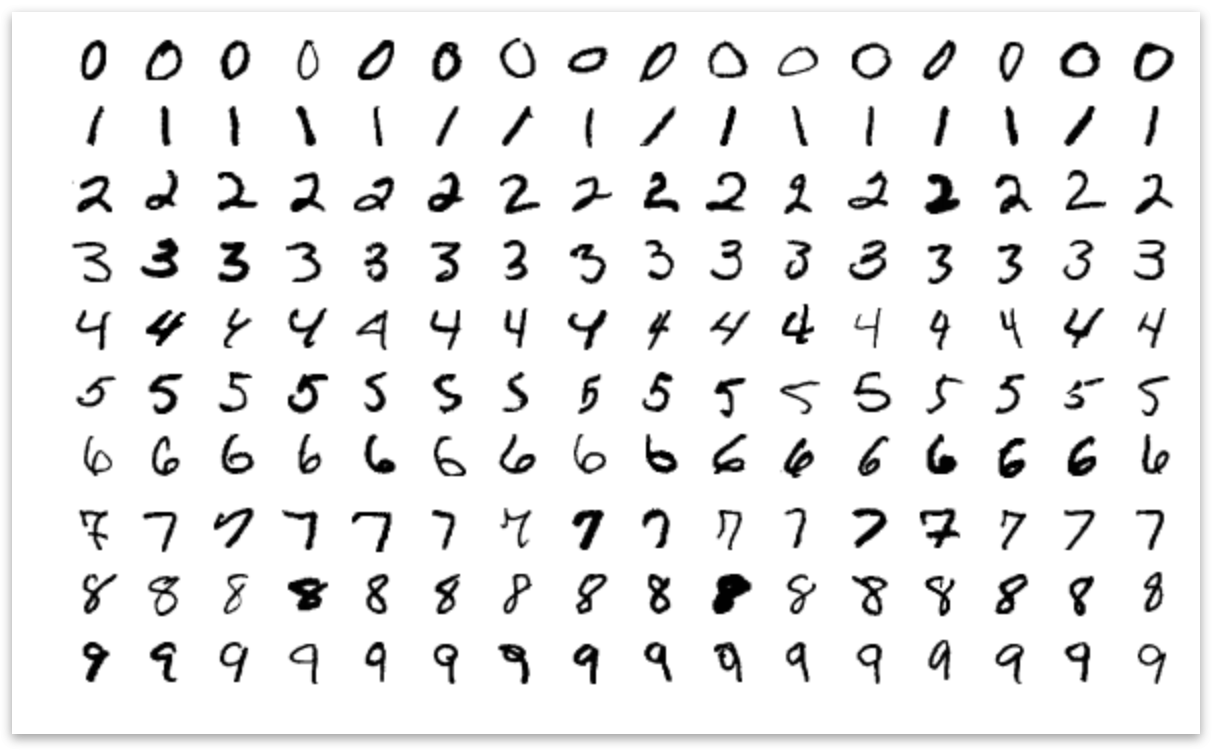
\includegraphics[width=0.5\textwidth]{Figures/DL/mnist.png}
  \caption[]{MNIST dataset example of handwritten digits.}
  \label{fig:mnist}
\end{figure}

The CNN was trained using the Radeon Vega Frontier Edition GPU, a top of the line graphics processor accelerator from AMD. This graphics card presents 8 levels of pairs of GPU Core frequency and voltage, Table \ref{tab:gpulevels}, that the GPU chooses in runtime accordingly to the temperature and power required, trying to maximize the performance. The GPU allows for the user definition of the frequency and voltage throw the ROCm System Management Interface - \textit{rocm-smi}. With it, a script was developed that performs undervoltage in steps of 10 mV on each of the 8 default voltage and frequency pairs. If the undervoltage is accepted by the software, the MNIST model is trained and after each run, the achieved accuracy is stored alongside the maximum power and average consumption, total energy consumed and the time that it took to execute the train.





\begin{algorithm}[H]
\SetAlgoLined
\KwResult{Write here the result }
 initialization\;
 \While{While condition}{
  instructions\;
  \eIf{condition}{
   instructions1\;
   instructions2\;
   }{
   instructions3\;
  }
 }
 \caption{How to write algorithms}
\end{algorithm}

\begin{figure}[!htb]
  \centering
  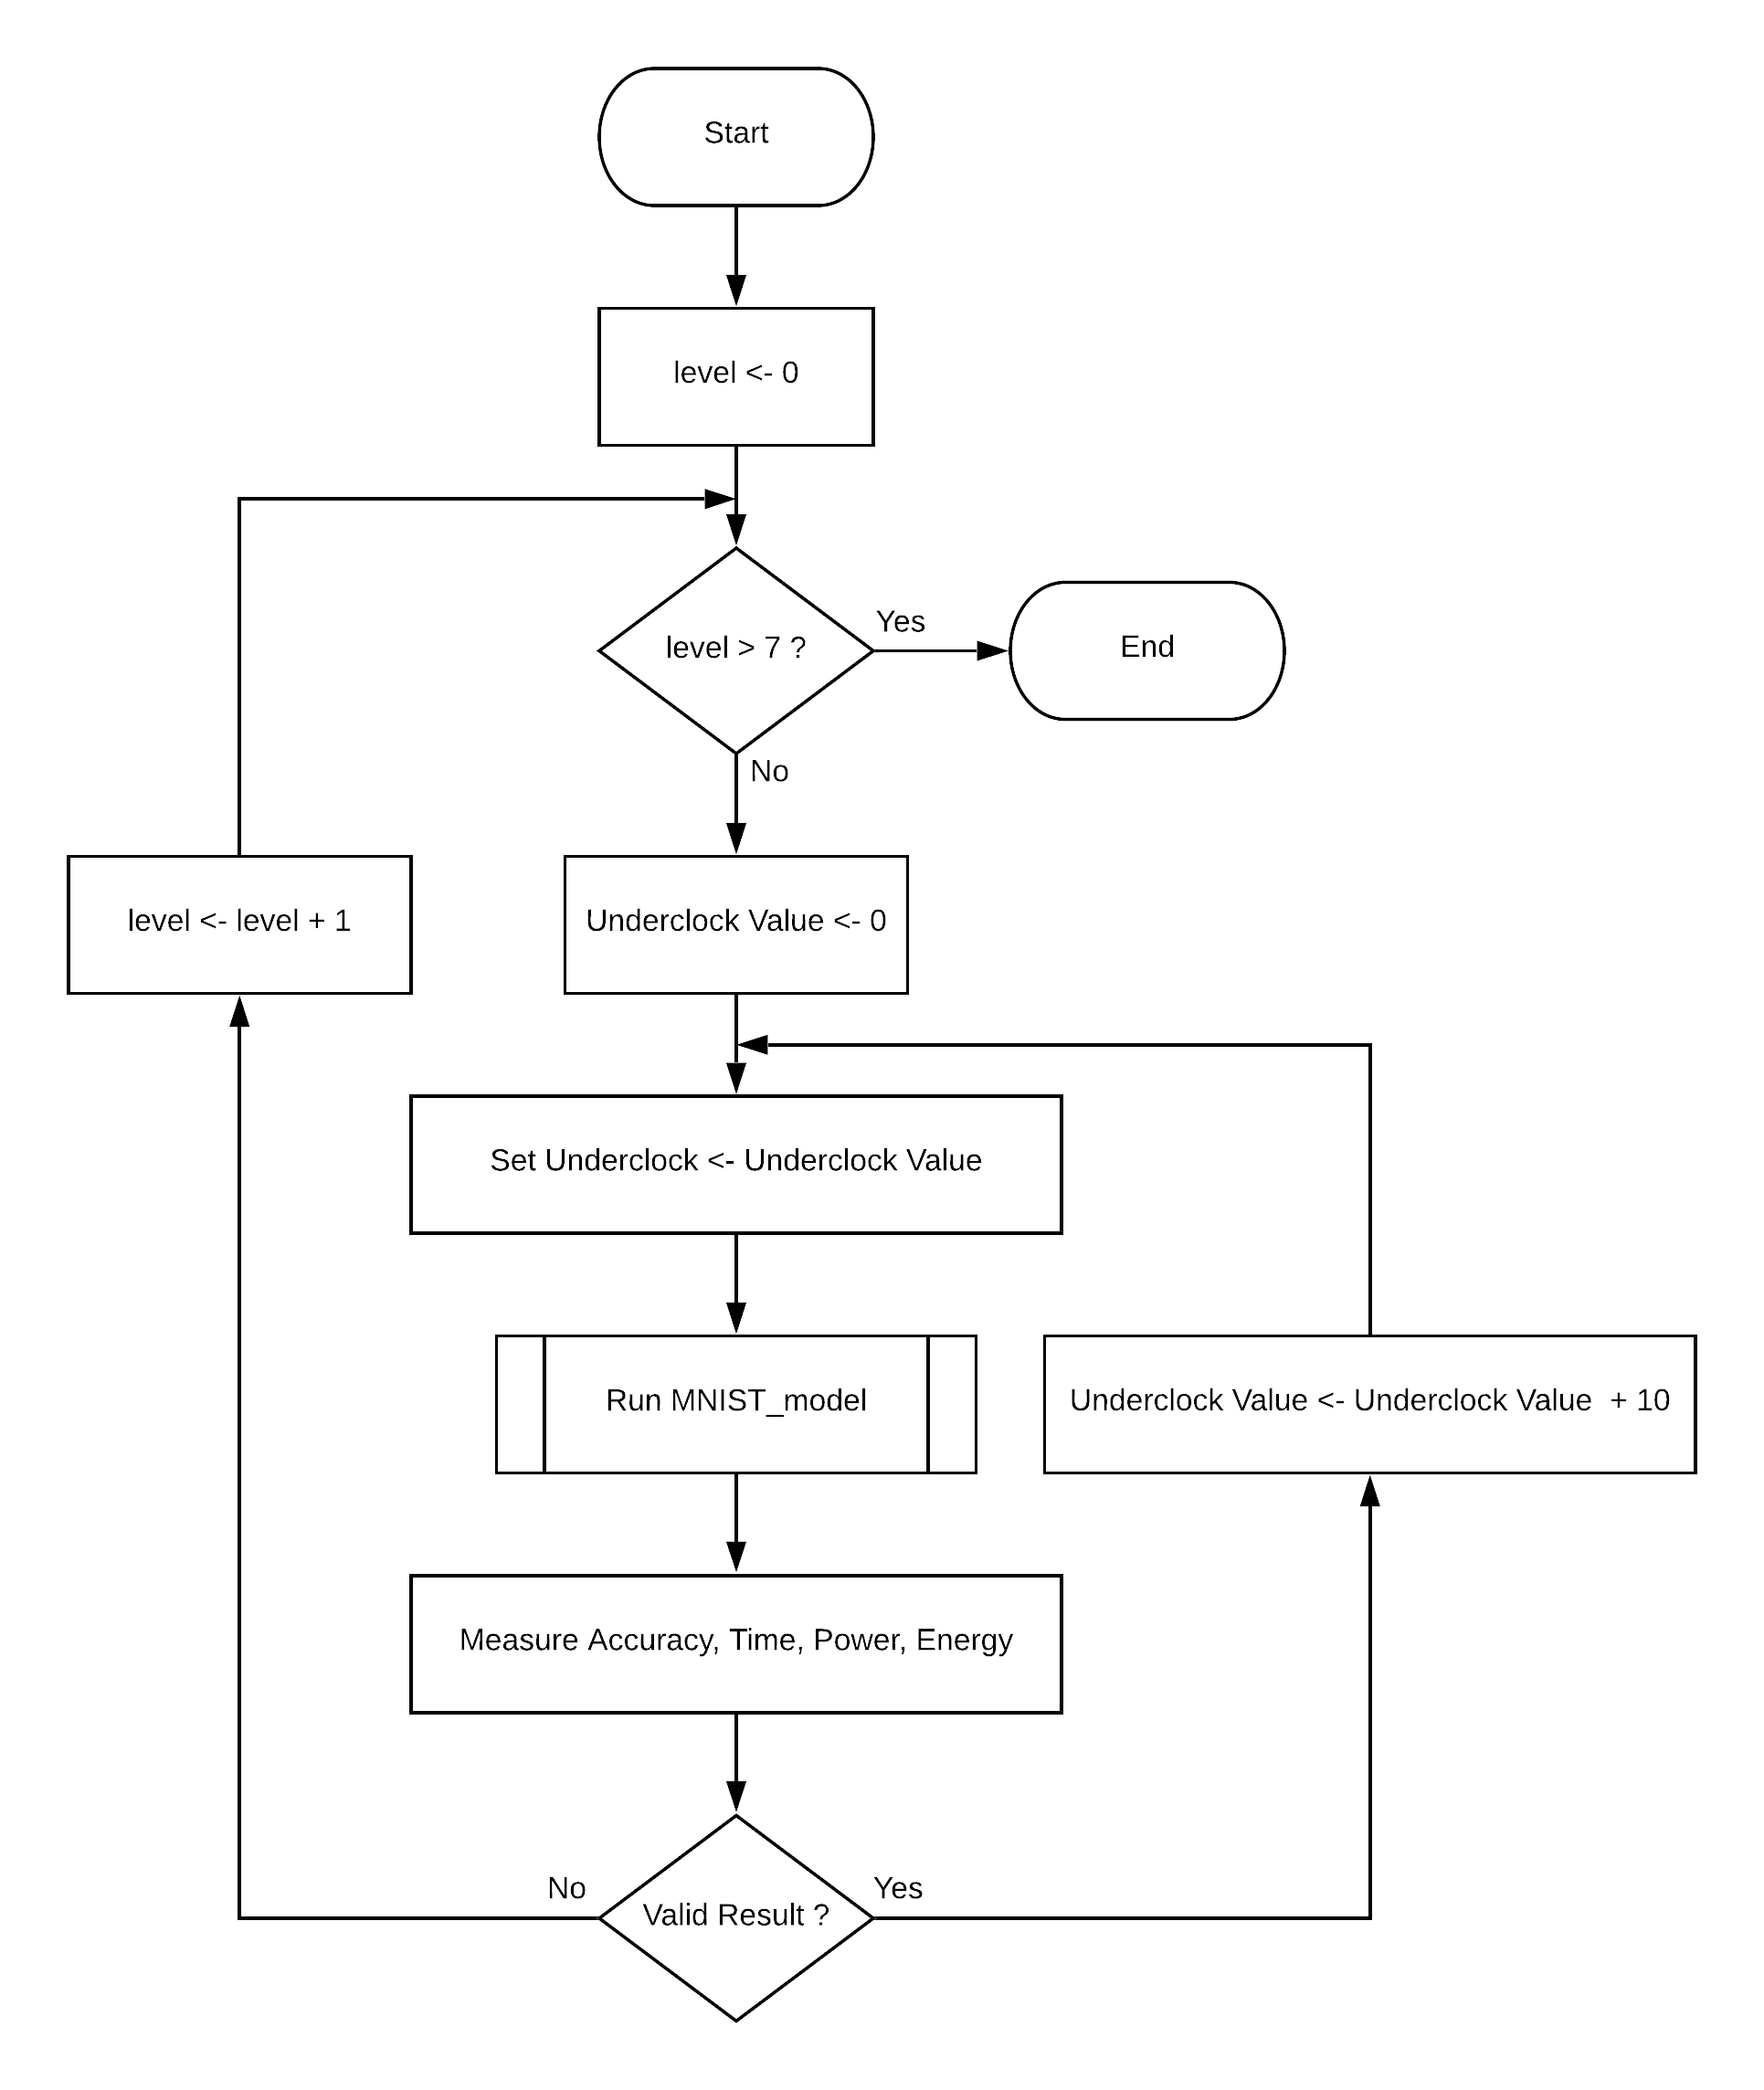
\includegraphics[width=0.75\textwidth]{Figures/DL/Underclock_Program.png}
  \caption[]{Flowchart of Automation Undervoltage Script.}
  \label{fig:undervoltage_program}
\end{figure}





\subsection{Preleminary Results}
\label{section:dvfseffects}

%%%%%%%%%%%%%%%%%%%%%%%%%%%%%%%%%%%%%%%%%%%%%%%%%%%%%%%%%%%%%%%%%%%%%%%%
\subsubsection{OverClock}
\label{section:underclock}

\subsubsection{UnderVoltage}




